\section{Examples} % (fold)
\label{sec:Examples}
This section shows some examples implemented with the
Sequence library to demonstrate its variable usage.
The following covers easy-to-understand and more sophisticated
examples. Consult the listed sources to understand the applications
thoroughly if something is unclear.

\subsection{Fibonacci Sequence}
\label{sub:Fibonacci Sequence}
This is an example of a specialized sequence constructor.
Listing~\ref{lst:fibonacci_sequence} shows the implementation of the Fibonacci 
sequence~\cite[p.~36]{math_diskrete_2011}:
\begin{lstlisting}[
  style=ES6, 
  caption=FibonacciSequence implementation,
  label={lst:fibonacci_sequence}
  ]
const start   = Pair(0)(1);
const whileFn =  _ => true;
const incrFn  = ([fst, snd]) => Pair(snd)(fst + snd);
/**
 * Generates the Fibonacci sequence.
 *
 * @constructor
 * @pure
 * @returns { SequenceType<Number> }
 *
 * @example
 * const result = take(8)(FibonacciSequence);
 *
 * console.log(...result);
 * // => Logs '1, 1, 2, 3, 5, 8, 13, 21'
 */
const FibonacciSequence = 
                    map(pair => pair(snd))(Sequence(start, whileFn, incrFn));
\end{lstlisting}
The |FibonacciSequence| constructor generates the Fibonacci sequence using the
|Sequence| and |Pair| constructors. The incrementation function produces a pair
containing the last returned value and the value to be returned.  The |map|
function then extracts the current Fibonacci number from the pair returned by
the sequence.

\subsection{Fizz Buzz}
\label{sub:Fizz Buzz}
Fizz Buzz is a simple game played with numbers, typically in a group setting. Players
take turns counting upward, but instead of saying numbers divisible by 3, they
say "Fizz", and instead of numbers divisible by 5, they say "Buzz". If a number
is divisible by both 3 and 5, they say "FizzBuzz". This game also serves as a 
programming task.
\newline
Frege Goodness~\cite{frege_goodness} includes a detailed explanation of the
game. 

First, let us look at the game's simplest form in listing~\ref{lst:simple_fizzbuzz}. 
The fizzes and buzzes are combined in a sequence. 
The sequence returns a number if neither a fizz nor a buzz occurs:

\begin{lstlisting}[
  style=ES6, 
  caption=Fizz Buzz example,
  label={lst:simple_fizzbuzz}
  ]
const limit    = 15;
const range    = Range(1, limit);
const fizzez   = cycle(["", "", "fizz"]);
const buzzez   = cycle(["", "", "", "", "buzz"]);

const pattern  = zipWith((fizz, buzz) => fizz + buzz)(fizzez)(buzzez);
const fizzbuzz = zipWith((num, str) => str === "" ? num : str)(range)(pattern);

console.log(...take(limit)(fizzbuzz));
// => Logs '1 2 "fizz" 4 "buzz" ... 11 "fizz" 13 14 "fizzbuzz"'
\end{lstlisting}

As you observe, the entire setup relies on sequences. We define three
distinct endless sequences. A range generates a line of numbers, while |cycle|
produces an unending repetition for "fizzes" and "buzzes". Memory usage remains
minimal. Subsequently, |zipWith| merges the individual sequences and yields a
new sequence. This uncomplicated setup underscores that working with sequences
is declarative, straightforward and highly understandable.

Now we are extending the application to add new rules during the runtime:

\begin{lstlisting}[
  style=ES6, 
  caption=Fizz Buzz example extended,
  label={lst:fizz_buzz}
  ]
import * as _ from "./src/sequence/sequence.js";

const infiniteNumbers = _.Sequence(1, _ => true, i => i + 1);

const createSequenceForRule = rule =>
  _.pipe(
    // add rule's text to number
    _.map(a => a === rule.getNr() ? rule.getText() : ""),     
    _.take(rule.getNr()), // abort on this rules number
    _.cycle
  )(infiniteNumbers);

const buildFizzBuzz = () => {
  const currentRules = model.rulesSnapshot().map(createSequenceForRule);
  const baseLine     = _.Sequence("", _ => true, _ => "");

  const fizzBuzz = _.pipe(
      // reduce to single sequence by combining all iterable values
    _.reduce$((acc, cur) => _.zipWith((a, b) => a + b)(acc)(cur), baseLine), 
    _.zipWith((numbers, pattern) => pattern === "" ? String(numbers) : pattern)
                 (infiniteNumbers), 
    // limit output
    _.take(model.getUpperBoundary()),
    _.drop(model.getLowerBoundary() -1),
  )(currentRules);

  model.setResult(fizzBuzz);
};
\end{lstlisting}
Listing~\ref{lst:fizz_buzz} shows two functions, |createSequenceForRule|, and
|buildFizzBuzz|. \\ 
|createSequenceForRule| is called with an argument |rule| representing a
number and a string. The returned infinite sequence then contains the
corresponding text at each multiple of the rules number. In the remaining
places, it contains an empty string. \\ 
Calling |createSequenceForRule(Rule(3, "fizz"))| thus creates a sequence
generating |"", "", "fizz", "", "", "fizz", ...|.\\
The function |buildFizzBuzz| reduces all sequences representing a rule to a
single sequence. 
Figures~\ref{fig:fizzbuzz_control} and \ref{fig:fizzbuzz_result} demonstrate a
screenshot of a simple application showing two rules and the resulting sequence.
The implementation enables adding new rules at runtime.

\begin{figure}[H] \centering \begin{minipage}{.5\textwidth} \centering
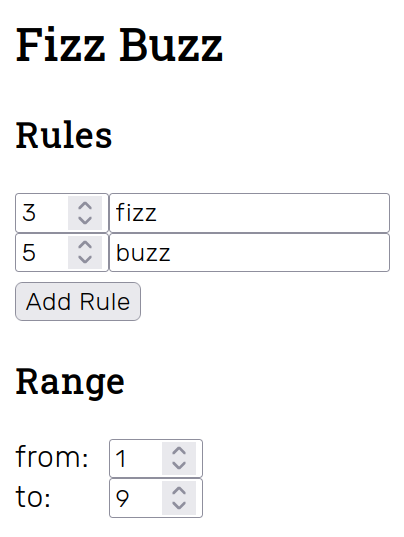
\includegraphics[width=.6\linewidth]{./mainmatter/pictures/fizzbuzz_control.png}
\captionof{figure}{Fizz Buzz controls} \label{fig:fizzbuzz_control}
\end{minipage}%
\begin{minipage}{.5\textwidth}
  \centering
  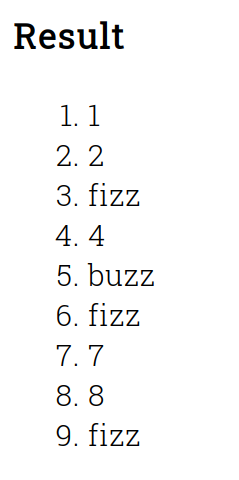
\includegraphics[width=.4\linewidth]{./mainmatter/pictures/fizzbuzz_result.png}
  \captionof{figure}{Fizz Buzz result}
  \label{fig:fizzbuzz_result}
\end{minipage}
\end{figure}

\subsection{JINQ}
\label{sub:results JINQ}
The following examples use JINQ to browse and process JSON files and to create
new sequences based on rules. At first glance, these two topics seem to have
nothing in common. However, as the following examples show, JINQ allows both
and therefore brings a general way to create and manipulate various data
structures.

\subsubsection{Find all Students}
\label{subsub:Find all Students}
We want to filter out all participants that have a student ID. As you can see
in the excerpt of the JSON file in listing~\ref{lst:json_file_devs}, the
property |switch-edu-id| is not defined for all people. Because the
|JsonMonad| works in the background with a maybe, such situations can be
processed without null handling.

\begin{lstlisting}[
  style=json, 
  caption=Excerpt of a JSON File including developers,
  label={lst:json_file_devs}
  ]
[
  {
    "id": 1,
    "name": "",
    "age": 28,
    "salary": 50000,
    "favoriteLanguages": [1, 3, 5]
  },
  {
    "id": 2,
    "switch-edu-id": "12-432-23",
    "name": "Emma Johnson",
    "age": null,
    "salary": 60000,
    "favoriteLanguages": [2, 4]
  },
  {
    "id": 3,
    "name": "Sophia Davis",
    "age": 40,
    "salary": null,
    "favoriteLanguages": [null, 4, 5]
  },
  ...
 ]
\end{lstlisting}

Using JINQ it is straightforward to access the desired students by just using
the function |where|:

\begin{lstlisting}[
  style=ES6, 
  caption=JINQ Example - find all students,
  label={lst:jinq_find_students}
  ]
const findAllStudentIds = developers => {
  const allIds =
    from(JsonMonad(developers))
      .select(x => x['switch-edu-id'])
      .result();
};
\end{lstlisting}

\subsubsection{Find Sophia's Programming Languages}
\label{subsub:Find Sophia's Programming Languages}

This example combines two JSON files. We use the JSON file from the previous
example and the one from listing~\ref{lst:json_file_lang} below.
Listing~\ref{lst:jinq_sophias_langs} shows the code that finds Sophia's 
favourite programming languages by combining two JSON files using |pairWith|. 

\begin{lstlisting}[
  style=json, 
  caption=Excerpt of a JSON File including programming languages,
  label={lst:json_file_lang}
  ]
[
  {
    "id": 1,
    "name": "Java"
  },
  ...
  {
    "id": 4,
    "name": "C++"
  },
  {
    "id": 5,
    "name": "Haskell"
  }
]
\end{lstlisting}
This is also comparatively easy to do with JINQ. |pairWith| allows adding a
second data source to the current one, forming all possible combinations. The
function |where| then keeps only the needed pairs. A simple mapping at the end
outputs the names of the programming languages.
\begin{lstlisting}[
  style=ES6, 
  caption=JINQ example - find Sophia's programming languages,
  label={lst:jinq_sophias_langs}
  ]
const sophiasProgrammingLanguages = (devs, languages) =>
    from(JsonMonad(devs))
      .where   ( dev    => dev.name === "Sophia Davis")
      .select  ( sophia => sophia.favoriteLanguages)
      .pairWith( JsonMonad(languages) )
      .where   ( ([langId, language]) => langId === language.id )
      .select  ( ([     _, language]) => language.name )
      .result  ();
\end{lstlisting}

\subsubsection{Pythagorean Triple}
\label{subsub:JINQ_Pythagorean Triple}
Listing~\ref{lst:triple} creates a new sequence containing the pythagorean
triples~\cite{pythagorean_triple} between 1 and 10:
\begin{lstlisting}[
  style=ES6, 
  caption=The Pythagorean Triple between 1 and 10,
  label={lst:triple}
  ]
import { Range, show } from "./src/sequence/sequence.js"
import { from }        from "./src/jinq/jinq.js";

const range = Range(1, 10);

const result =
  from(range)
    .pairWith(range)
    .pairWith(range)
    .where ( ([ [a,b], c ]) => a * a + b * b === c * c)
    .select( ([ [a,b], c ]) => `[${a}, ${b}, ${c}]`)
    .result();

console.log(show(/** @type SequenceType */ result));
// => Logs '[[3, 4, 5],[4, 3, 5],[6, 8, 10],[8, 6, 10]]
\end{lstlisting}
\subsection{Numerical Differentiation}
\label{sub:Numerical Differentiation}
This example shows a mathematical use case, the numerical differentiation using
sequences:

\begin{lstlisting}[
  style=ES6, 
  caption=Differentiation using sequences,
  label={lst:diff_sequences}
  ]
const halve   = x => x / 2;
const repeatF = (f, x) => _.Sequence(x, _ => true, f);
const halves = h0 => repeatF( halve, h0);

const slope = f => x => h => (f(x + h) - f(x)) / h;
const differentiate = h0 => f => x => _.map ( slope(f)(x) ) (halves(h0));
\end{lstlisting}

Listing~\ref{lst:diff_sequences} implements the following steps: 


\begin{itemize}
  \item{|repeatF| repeatedly applies the function $f$ to a value of the
    previous calculated result, starting with $x$.}
  \item{ |halves| is using |repeatF| and |halve| to halve a value $h0$.} 
    \item{|slope| calculates the slope of a function $f$ at the position $x$
      with delta $h$.}
 \end{itemize}

This code already provides everything needed for differentiation. The function
|differentiate| calculates the slope of a function at a given point $x$ more
and more exactly.
Listing~\ref{lst:diff_seq_parabola} uses these functions to determine the 
slope at $x = 1$ of the function |parabola| defined on line~\ref{line:diffs}:

\begin{lstlisting}[
  style=ES6, 
  caption=Differentiation using sequences,
  label={lst:diff_seq_parabola}
  ]
const parabola = x => x * x; *'\label{line:diffs}'*

const diffs = differentiate(0.5)(parabola)(1);
\end{lstlisting}

Since |diffs| contains an infinite sequence, one further
function is still needed.
Listing~\ref{lst:impl_within} shows the function |within|, which allows
differentiating until two successive values are smaller than a given epsilon:

\begin{lstlisting}[
  style=ES6, 
  caption=Implementation of within,
  label={lst:impl_within}
  ]
const within = eps => sequence => {
  const [a, rest] = _.uncons(sequence);
  const [b]       = _.uncons(rest);
  const diff      = Math.abs(a - b);

  if (diff <= eps) return b;
  return within(eps)(rest);
};
const slopeOfFAtX = within(0.000_1)(diffs);
\end{lstlisting}

Listing~\ref{lst:impl_within} defines the following implementations:

\begin{itemize}
  \item |within| calculates recursively the slope of the |parabola| using the
    sequence |diffs| until a satisfying accuracy. Because of the laziness of
    the sequence, |within| only calculates as many slopes as needed.
  \item At the end, |slopeOfFAtX| calculates the slope with the given parameters.
\end{itemize}


\subsection{Tic Tac Toe with a Kind of AI}
\label{sub:Alpha - Beta Algorithm}
This section describes the implementation of the alpha-beta heuristic in
JavaScript, an algorithm for estimating how good a position a game player is
in. \\ 
This algorithm allows for building a computer-controlled opponent for a
turn-based game. Hughes explains how the algorithm uses laziness and
higher-order functions to be modular and extensible in his paper.~\cite[p.
16]{hughes_why_1989}. As chapter~\ref{chap:Modularizing Programs} describes, the
Sequence library supports these two concepts, thus allowing to port the
algorithm to JavaScript.

\subsubsection{How does the Algorithm work?} % (fold)
\label{subsub:How does the Algorithm work?}
The following explanation is meant to give a brief overview for the
algorithm, allowing to understand the preceding code. For a deeper
understanding of the algorithm, consider ~\cite[Ch. 5]{hughes_why_1989} or the
section "Incremental Development" in Frege Goodness~\cite{frege_goodness}.

\paragraph{Building a Game Tree} The idea of the algorithm is to build a tree
containing \textit{all} possible playing fields. The start node in this
tree is the current state of the playing field. Its children are all possible
playing fields, which can arise when the players make their next moves. This
results in a potentially endless tree. All direct successors of a node are the
next possible moves for this node's playing field. Since this tree can be huge,
depending on the game, even infinitely large, only a lazy data structure can
handle it.\\
The algorithm must estimate whether a playfield is good or bad for a player to
find the best possible next move. The simplest way to figure this out is to
look at the playing field and decide if a player has already won. In the case
of tic tac toe, a player has won when three of his symbols are next to each
other. \\
A function (called |evalFunction|) does this evaluation - if the algorithm has
won the game on a field, it evaluates to 1 if it has lost to -1, in all other
cases, to 0.\\
The |evalFunction| is mapped over the tree (where higher-order functions come
into play) - each node is assigned its static value, saying how promising the
playfield of this node is. This results in a new tree with the value of
|evalFunction| assigned to the nodes instead of all possible fields.\\

\paragraph{What is the best Move?}
The tree's root is the current playing field - the algorithm cannot know from
the root which moves are good and which are not. The previously mentioned
|evalFunction| will evaluate to 0 for most nodes directly after the root.
Therefore, the computer also calculates subsequent moves. The values of the
lowest calculated nodes are then propagated upwards to the root. 

The function |maximize| goes through to the lowest precalculated level. It
evaluates the board there: when it is the computer's turn, it selects the board with
the highest value assigned (safest chance of winning). If it is the opponent's
turn, it selects the smallest value (the algorithm thus assumes that the
opponent also selects the best possible move). This found value is assigned to
the parent node as a result - and chooses the best move on this level according
to the same scheme. Ultimately, the root has the value with the best possible
chances of winning.

\paragraph{How to evaluate the huge Tree?} The tree of possible moves and possible
result values can be huge. So the algorithm must have a way to limit the tree
to a fixed depth. The algorithm uses pruning - from a freely selectable depth,
it cuts the children off. 

\subsubsection{Implementation}
\label{subsub:alphabeta_implementation}
\paragraph{Basic Types and Helper functions} 
Listing~\ref{lst:tictactoe_types} shows the required types for the game
implementation. \\
A pair models the |Tree| (line~\ref{line:ttt_treetype}) - the first
value is the current node, and the second value is a sequence consisting of
further trees. The types |Player| and |Stone| exist only for writing more
expressive JSDoc.

\begin{lstlisting}[
  style=ES6, 
  caption=Tic tac toe types,
  label={lst:tictactoe_types}
  ]
/**
 * 
 * @template _T_
 * @typedef {SequenceType<Tree<_T_>>} TreeSequence
 */

/** *'\label{line:ttt_treetype}'*
 * @template _T_
 * @typedef { PairSelectorType<_T_, TreeSequence<_T_>> } Tree
 */


/**
 * @typedef { "Computer" | "Human" | "NoPlayer" } Player
 */

/**
 * @typedef { 1 | -1 | 0 } Stone
 */

/**
 * @typedef Board
 * @property { Player } whosTurn
 * @property { Iterable<Stone>} fields - A board has fields from 0 to 8.
 */
\end{lstlisting}

Listing~\ref{lst:tictactoe_players} includes the definition of the players and some
functions used in the game process. Since JavaScript does not support pattern
matching, the functions |opponent| and |stone| use a workaround - they store
the mappings in an object.

\begin{lstlisting}[
  style=ES6, 
  caption=The players and some helper functions,
  label={lst:tictactoe_players}
  ]
/** @type { Player } */
const Computer = "Computer";

/** @type { Player } */
const Human = "Human";

/** @type { Player } */
const NoPlayer = "NoPlayer";

/**
 * Returns the opponent of a given player.
 * @param { Player } player
 * @return Player
 */
const opponent = player => {
  const pairings = {
    "Computer" : Human,
    "Human"    : Computer,
    "NoPlayer" : NoPlayer,
  };
  return pairings[player];
};

/**
 * Returns the stone number of a given player.
 * @param { Player } player
 * @returns Stone
 */
const stone = player => {
  const pairings = {
    "Computer" :  1,
    "Human"    : -1,
    "NoPlayer" :  0,
  };
 return pairings[player];
};

/**
 * Transforms each board element using the given function f.
 * @template _T_, _U_
 * @type {
 *         (f: (Board) => _T_)
 *      => (tree: Tree<_U_>)
 *      => Tree<_T_>
 * }
 */
const treeMap = f => ([a, sub]) => Pair(f(a))(map(treeMap(f))(sub));
\end{lstlisting}

\paragraph{Building trees and processing the Game Board} 
Listing~\ref{lst:tictactoe_gametree} shows the functions for building a game
tree. |unfold| is a function that takes a value (for example, a board) and
creates new values of the same types of it (for example, all boards possibly
arising in one move).
\begin{lstlisting}[
  style=ES6, 
  caption=Tic tac toe game tree,
  label={lst:tictactoe_gametree}
  ]
/**
 * Generates recursively a game tree, which is potentially endless.
 * @template _T_
 * @type {
 *       (unfold: ((_T_) => Iterable<_T_>))
 *    => (a: _T_)
 *    => Tree<_T_>
 * }
 */
const buildTree = unfold => a => {
  const as = unfold(a);
  const children = map(buildTree(unfold))(as);
  return Pair(a)(children);
};

/**
 * Creates a game tree.
 * @param { Board } board
 * @returns Tree<Board>
 */
const gameTree = board => buildTree(moves)(board);
\end{lstlisting}

Listing~\ref{lst:tictactoe_move} includes the |moves| function. This function
calculates all possible moves for a player based on the current playing field.
If a player has already won, it returns an empty sequence.
\begin{lstlisting}[
  style=ES6, 
  caption=Tic tac toe move function,
  label={lst:tictactoe_move}
  ]
/**
 * Indexes each field using a {@link PairType}.
 * @param { Iterable<Stone> } fields
 * @return { SequenceType<PairType<Stone, Number>> }
 */
const indexFields = fields => zip(fields)(Range(1,9));

/**
 * Calculates possible moves for a given board.
 * @param { Board } board
 * @return SequenceType<Board>
 */
const moves = board => {
  if (hasWon(board)(Computer)) return /**@type {SequenceType<Board>} */nil;
  if (hasWon(board)(Human))    return /**@type {SequenceType<Board>} */nil;

  const otherPlayer   = opponent(board.whosTurn);
  const indexedFields = indexFields(board.fields);

  const blankIndices =
    from(indexedFields)
      .where( ([content, _]) => content === stone(NoPlayer))
      .select( ([_, i]) => i)
      .result();

  const fieldsWithPlayerPlacedAt = pos =>
    from(indexedFields)
      .select(([content, i]) => i === pos ? stone(board.whosTurn) : content)
      .result();

  const boardFieldsAfterMove = map (fieldsWithPlayerPlacedAt) (blankIndices);

  return map(fields => ({fields, whosTurn: otherPlayer})) (boardFieldsAfterMove);
};
\end{lstlisting}

\paragraph{Evaluating a Board}
Listing~\ref{lst:tictactoe_hasWon} shows the implementation of the |hasWon|
function, which checks if a player has won on a given board. The evaluation
function, explained in section ~\ref{subsub:How does the Algorithm work?}, uses
this function to assess a playing field. Line~\ref{line:ttt_static_eval}
defines this function called |staticEval|.

\begin{lstlisting}[
  style=ES6, 
  caption=Tic tac toe hasWon function,
  label={lst:tictactoe_hasWon}
  ]
/**
 * Checks, if a player has won.
 * @type {
 *    (board: Board)
 *    => (player: Player)
 *    => Boolean
 * }
 */
const hasWon = board => player => {
  const winTriples = [
    [1,2,3], [4,5,6], [7,8,9], // row
    [1,4,7], [2,5,8], [3,6,9], // col
    [1,5,9], [3,5,7]           // diag
  ];

  const checkTriple = triple => {
    const actualStone   = stone(player);
    const indexedFields = indexFields(board.fields);

    const playerOnFields =
      from(indexedFields)
      .where( ([_, i])        => triple.includes(i))
      .select( ([content, _]) => content === actualStone)
      .result();

    return foldl$((acc, cur) => acc && cur, true)(playerOnFields);
  };
  return pipe(
    map(checkTriple),
    foldl$((acc, cur) => acc || cur, false)
  )(winTriples)
};

/**
 * Evaluates a given board.
 * @param { Board } board
 * @returns Number
 */
const staticEval = board => {*'\label{line:ttt_static_eval}'*
  if (hasWon (board) (Computer)) return 1.0;
  if (hasWon (board) (Human))    return -1.0;
  return 0.0;
};

\end{lstlisting}

\paragraph{Finding the best Move}
Listing~\ref{lst:tictactoe_minimax} shows the implementation of the functions
|maximize| (and its counterpart |minimize|) explained in
section~\ref{subsub:How does the Algorithm work?}. These functions determine
which are the best moves.

\begin{lstlisting}[
  style=ES6, 
  caption=Tic tac toe minimax algorithmus,
  label={lst:tictactoe_minimax}
  ]
/**
 * Determines the best move.
 * @template _T_
 * @param { Tree<_T_>}
 * @return { _T_ }
 */
const maximize = ([a, sub]) => {
  if (sub ["=="] (nil)) return a;
  return max$ (map(minimize)(sub))
};

/**
 * Determines the best move for the opponent.
 * @template _T_
 * @param { Tree<_T_>}
 * @return { _T_ }
 */
const minimize = ([a, sub]) => {
  if (sub ["=="] (nil)) return a;
  return min$ (map(maximize)(sub))
};
\end{lstlisting}

\paragraph{Pruning Trees} 
We cut off (prune) the possibly infinite tree. The following
listing~\ref{lst:tictactoe_prune} shows the implementation of this pruning.
Since subtrees are sequences, |nil| replaces them when pruning.

\begin{lstlisting}[
  style=ES6, 
  caption=Tic tac toe prune function,
  label={lst:tictactoe_prune}
  ]
/**
 * Prunes a given {@link Tree} to a max depth n.
 * @template _T_
 * @type {
 *           (n: Number)
 *        => (tree: Tree<_T_>)
 *        => Tree<_T_>
 * }
 * @param n
 */
const prune = n => tree => {
  const [a, sub] = tree;
  if (n === 0) return Pair(a)(nil);
  else return Pair(a)(map(prune(n-1))(sub));
};
\end{lstlisting}

\paragraph{Putting it all together}
The following functions evaluate a playing field. \\ 
The function |nextBoard| calculates the best possible next move for the
computer. The number |lookaheads| defines how many turns the algorithm
calculates in advance. Based on these calculations the algorithm chooses the
next move.

\begin{lstlisting}[
  style=ES6, 
  caption=Tic tac toe - evaluating functions,
  label={lst:tictactoe_eval}
  ]
/**
 * Evaluates a given Board by building a tree
 * @type {
 *            (lookahead: Number)
 *         => (board: Board)
 *         => Number
 * }
 */
const evaluate = lookahead => board => {
  const prunedTree = prune(lookahead)(gameTree(board));
  const mappedTree = treeMap(staticEval)(prunedTree);
  return minimize(mappedTree);
};

/**
 * @template _T_
 * @type {
 *            (lookahead: Number)
 *         => (board: Board)
 *         => PairSelectorType<_T_, Board>
 * }
 */
const nowValue = lookahead => board =>
  Pair(evaluate(lookahead)(board))(board);

/**
 * Calculates the next board with given board fields.
 * @type {
 *          (lookahead: Number)
 *       => (inFields: Array<Number>)
 *       => Board
 * }
 */
const nextBoard = lookahead => inFields => {
  const currentBoard = { whosTurn: Computer, fields: inFields };
  // get all possible
  const possibleMoves  = moves (currentBoard);
  if (isEmpty(possibleMoves)) return currentBoard;
  // evaluate each move by looking ahead how good it is
  let evaluatedMoves =  map (nowValue(lookahead)) (possibleMoves);

  // if the computer is sure to lose 
  // only look one place ahead to prevent the "nearest" loss
  if (onlyLoses(evaluatedMoves)) {
    evaluatedMoves = map (nowValue(1)) (possibleMoves);
  }

  /**
   * Gets the highest ranked board of the passed board
   * @param {SequenceType<PairSelectorType<Number, Board>>} boards
   * @return Board
   */
  return bestOf(evaluatedMoves);
};
\end{lstlisting}

\subsubsection{The Result} % (fold)
\label{sec:ttt_result}
One advantage of JavaScript is that it works hand in hand with websites and
HTML. A website with a UI (like figure~\ref{img:ttt_playfield}) can now use the
algorithm:\\

\begin{figure}[H]
    \centering
    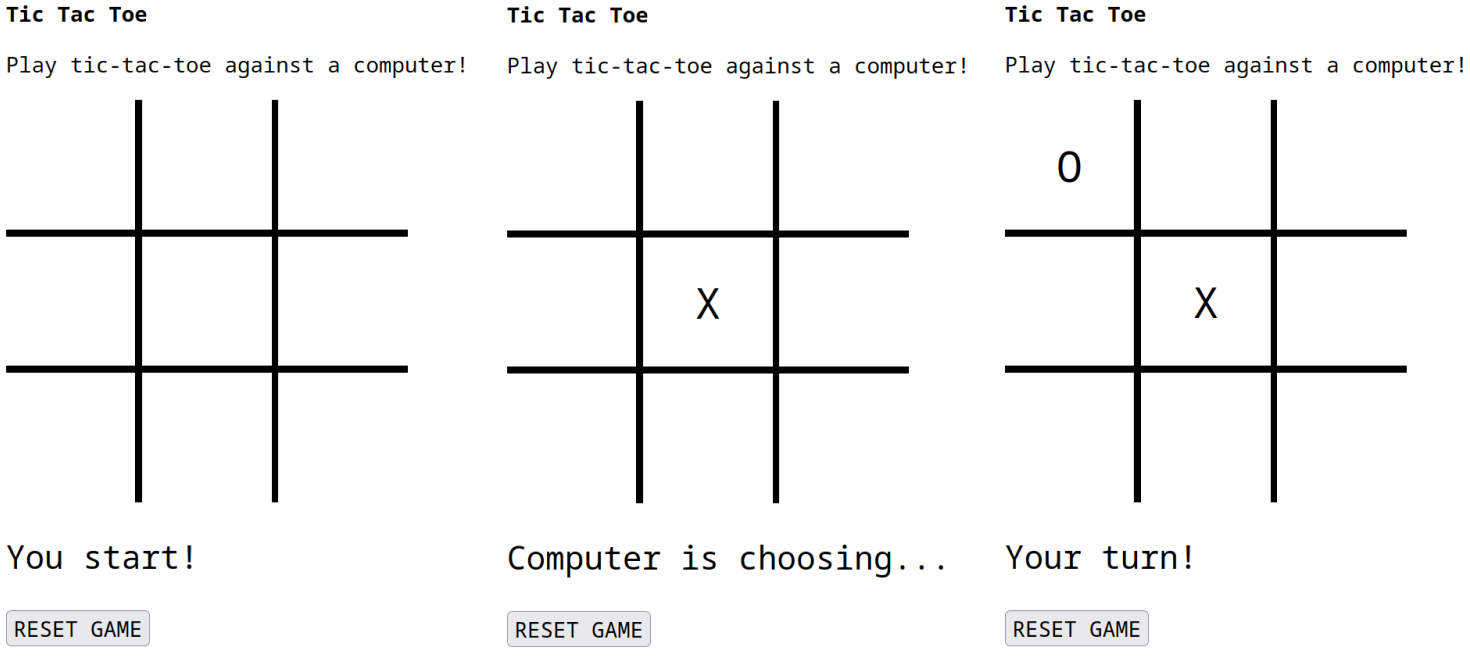
\includegraphics[width=0.9\textwidth]{./mainmatter/pictures/tic-tac-toe-field.png}
    \caption{A website using the algorithm}
    \label{img:ttt_playfield}
\end{figure}

When a player places his stone on the board, the function |nextBoard| gets
called. The algorithm automatically makes the best possible next turn based on
how many moves it can look ahead and returns the new board.
% subsubsection The result (end)

\subsubsection{Conclusion} % (fold)
\label{subsub:ttt_conclusion}
This example shows impressively how the Sequence library enables developers to
adapt an algorithm developed for functional programming languages in
JavaScript.\\
Of course, copying the algorithm is impossible because JavaScript misses some
language features like pattern matching. Nevertheless, the essential concepts
and logic of the algorithm can be adopted directly. \\
It is also exciting how JSDoc allows constructing straightforward talking types
like |Player| or |Stone| (listing~\ref{lst:tictactoe_types}).\\
To extend the algorithm, for example, to improve the static evaluation to
decide how good a current playing field is, only one function has to be
adjusted. Also, the evaluation of the algorithm can be easily improved and
detached from other logic by increasing the number of lookahead moves. Further
optimizations to prune away subtrees that are out of consideration anyway can
be done directly in the function |maximize|.\\
Thus, the modularity and extensibility of the program is very high.
% subsubsection Conclusion (end)
